\documentclass[11pt,a4paper,landscape]{article}
\usepackage{float}
\usepackage{graphicx}
\usepackage{hyperref}
\usepackage{multicol}
\setlength\columnsep{2em}
\usepackage[utf8]{inputenc}
\usepackage[czech]{babel}
\usepackage[left=2cm,right=2cm,top=2cm]{geometry}
\pagestyle{empty}
 
\begin{document}
{
\noindent
\Large{\textbf{IDS 2022/2023\,--\,1.~část projektu}} \\ \normalsize
Adam Mrkva (\verb|xmrkva04|), Matyáš Strelec (\verb|xstrel03|)}

\begin{multicols*}{2}

\section{Zadání}

\subsection*{Rezervace letenek}

Vaším úkolem je navrhnout webovou aplikaci pro rezervaci letenek. Systém musí uživateli umožnit specifikovat požadavek pomocí místa odletu a příletu, data, času, třídy, letecké společnosti apod. Jedno letadlo může létat na více letech, stejně tak mezi dvěmi destinacemi může létat více letadel různých společností.

Zákazník si rezervuje letenku, která může být na několik letů, i různých společností (např. letenka Praha $\rightarrow$ San Francisco s lety Praha $\rightarrow$ Londýn ČSA, Londýn $\rightarrow$ San Francisco British Airways). Systém musí umožnit klientovi tisk letového itineráře, který obsahuje informace o dobách příletů a odletů na jednotlivých letištích.

Každý typ letadla má různý počet sedadel a jejich rozvržení do tříd. Nemodelujte jednotlivá sedadla. Rezervací může klient zamluvit i více míst v jednom letu. Technická mezipřistání modelovat nemusíte. Systém musí evidovat, která společnost kdy, odkud a kam létá. Cena sedadla v dané třídě může být u každé společnosti jiná, cena letenky je dána součtem cen všech rezervovaných sedadel na všech letech. Pokud klient rezervovanou letenku včas nezaplatí, rezervace se z databáze smaže. 

\section{Popis datového modelu}

\subsection{ER diagram}
ER diagram obsahuje tyto entity:

\textbf{Let:}

\textbf{Letadlo:}

\textbf{Společnost:}

\textbf{Letiště:}

\textbf{Letový režim:}

\textbf{Košík:}

\textbf{Datum:}

 
\subsection{Diagram případů užití}
V diagramu případů užití figuruje několik aktérů.

\textbf{Čas:} systém tedy po uplnyutí určité doby může smazat neuhrazenou rezervaci.

\textbf{Anonymní uživatel:} může se registrovat, čímž se z něj stane klient. Může také vytvořit rezervaci, k čemuž je potřeba zobrazit lety dle daných požadavků. Může tisknout nějaký letový itinerář. Rezervaci může uhradit.

\textbf{Klient:} je rozšířením anonymního uživatele, tedy může vše co on, navíc může své rezervace zrušit, nebo zobrazit – lze zobrazit rezervace buď uhrazené nebo neuhrazené.

\textbf{Správce:} je rozšířením klienta. Navíc může spravovat uživatele (přidat a blokovat), společnosti (přidat ji), letový režim (upravit ho), či autorizovat nějakou operaci v systému.

\end{multicols*}

\begin{center}
\begin{figure}[H]
        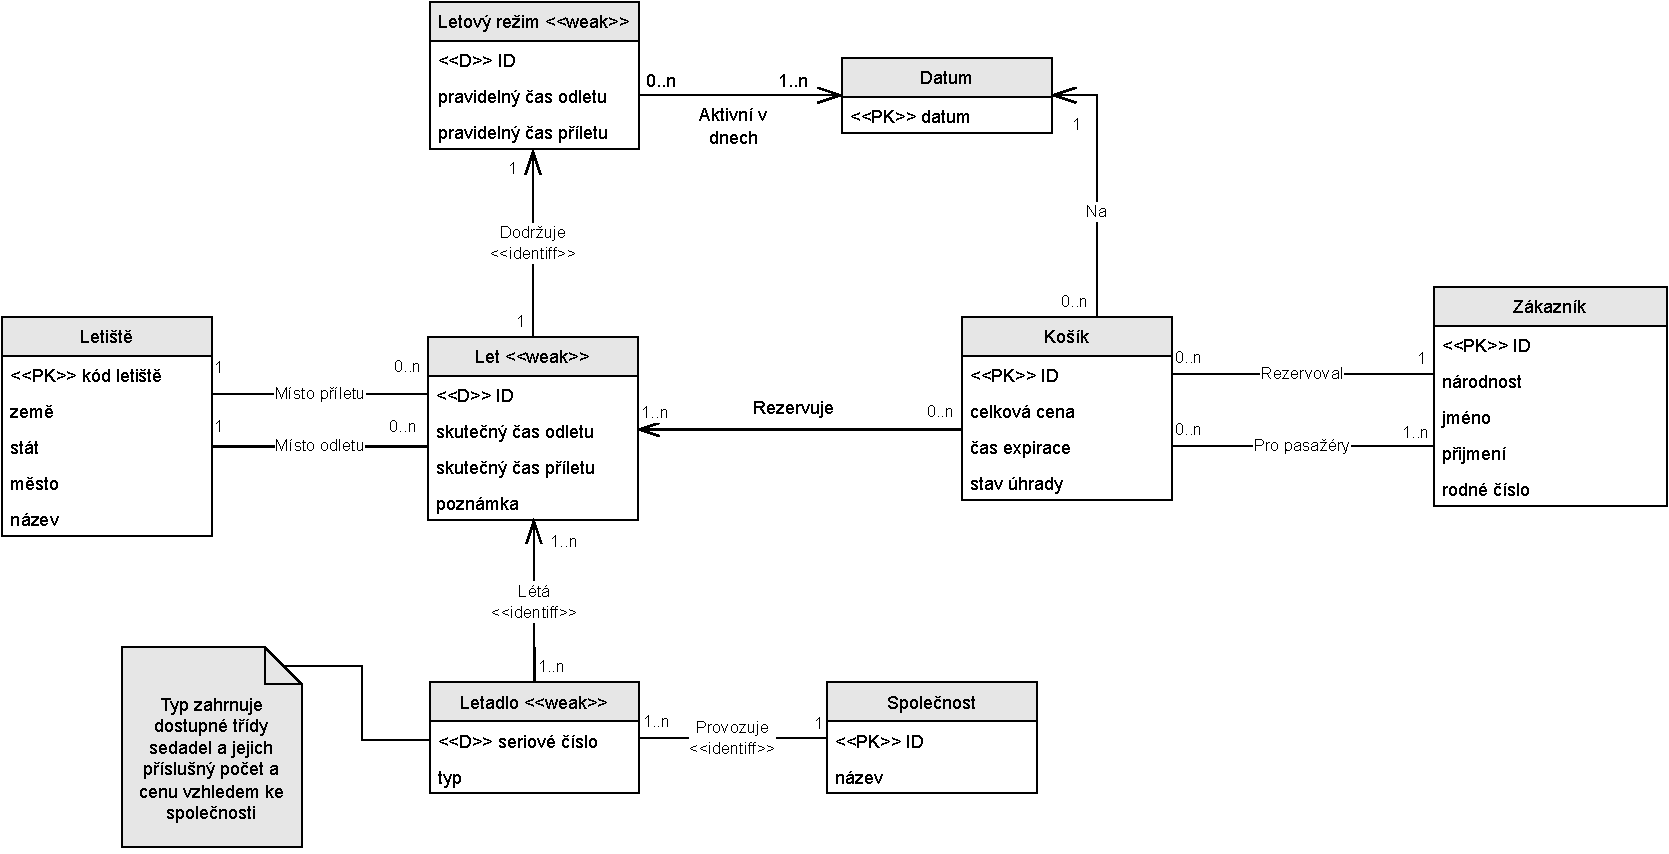
\includegraphics[scale=0.85]{diagrams/er-diagram.pdf}
        \caption{ER diagram}
        \label{fig:1}
\end{figure}
\begin{figure}[H]
        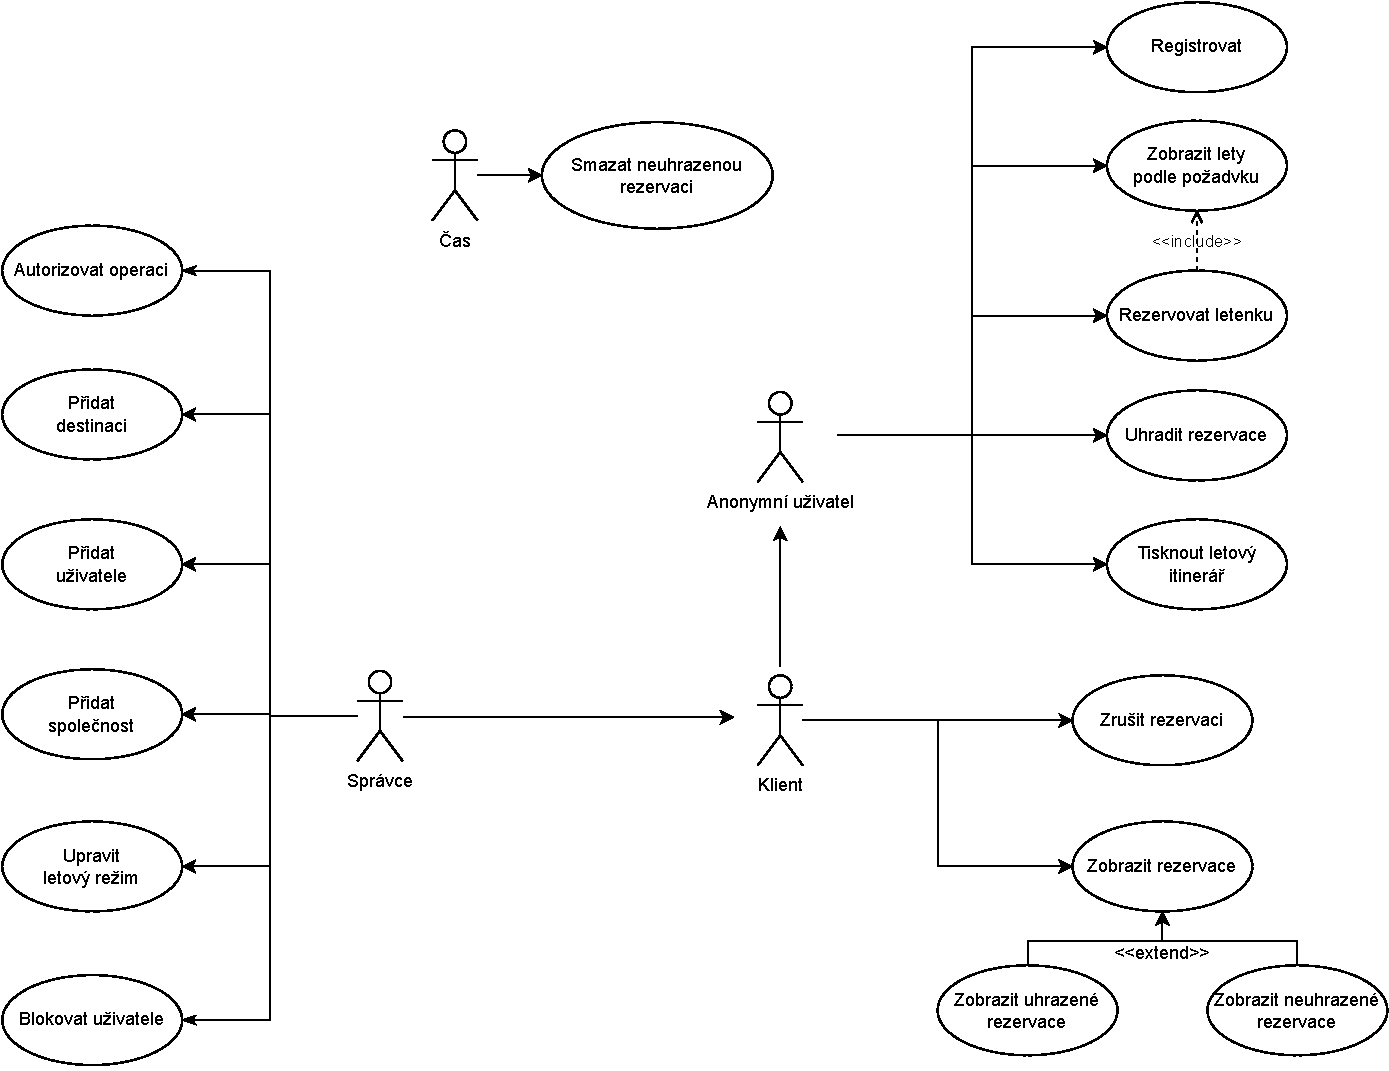
\includegraphics[scale=0.85]{diagrams/usecase-diagram.pdf}
        \caption{Diagram případů užití}
        \label{fig:2}
\end{figure}
\end{center}

\let\clearpage\relax

\end{document}